\section{NatureGym}
\label{sec:naturegym}
We introduce \textbf{NatureGym}, a pipeline that turns a published Nature-family paper into a ready-to-run agentic task.
Each task is a containerized package comprising a task brief, the dataset, a held-out test set, an automated evaluator, and a SOTA anchor score.
NatureGym standardizes papers with heterogeneous formats, toolchains, and data modalities into one reproducible task format, while imposing an information firewall that withholds the original method so that agents must discover solutions rather than reproduce them.


\subsection{Pipeline Overview}
\label{sec:gym:overview}


\begin{figure}[t]
    \centering
    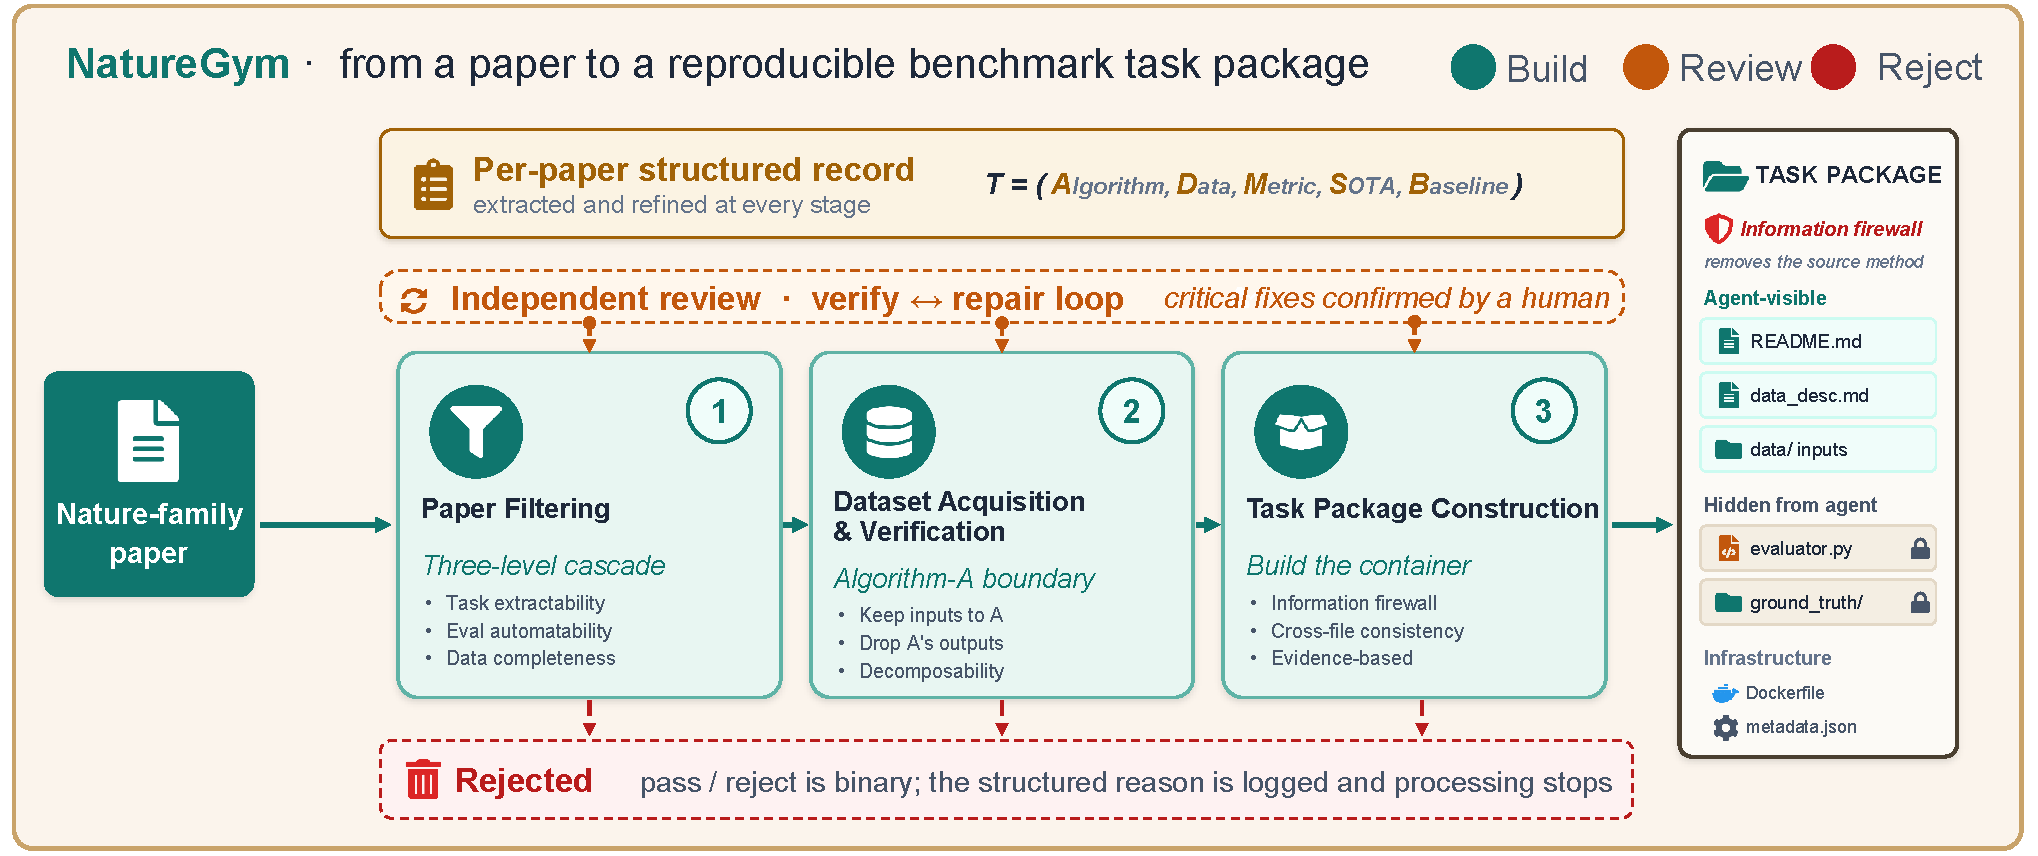
\includegraphics[width=1.0\linewidth]{figures/naturegym_v3.pdf}
    \caption{
    \textbf{The NatureGym pipeline.} Three review-gated stages turn one Nature-family paper into a containerized task package, refining a shared per-paper record $T=(A,D,M,S,B)$ along the way. An information firewall removes the source method, so the agent receives only dataset inputs, task brief, and a held-out test set, and tries to discover rather than reproduce.
    }
    \label{fig:gym-pipeline}
\end{figure}

As shown in Fig.~\ref{fig:gym-pipeline}, NatureGym builds each task through three stages: Paper Filtering (\S\ref{sec:gym:filter}), Dataset Acquisition and Verification (\S\ref{sec:gym:data}), and Task Package Construction (\S\ref{sec:gym:build}).
Each stage ends with an independent review that catches and corrects errors through a verify--repair loop before the next stage begins.

Every stage serves two purposes. First, it makes a binary pass-or-reject decision, terminating all downstream processing for rejected papers. Second, it extracts and refines structured task information into a per-paper record that accumulates across stages, so that task package construction can consume this record directly without re-reading the paper.

We represent each task as a tuple $T=(A,D,M,S,B)$, namely a core algorithm $A$, a dataset $D$, a metric $M$, a SOTA score $S$, and an optional baseline $B$.
The pipeline starts to fill in this tuple at the filtering stage and refines it in every later stage.
Every stage is run by an LLM agent, and a human confirms the critical corrections that each review surfaces.


\subsection{Paper Filtering}
\label{sec:gym:filter}


Paper filtering identifies candidate papers suitable for task construction through three steps: preprocessing, a three-level cascade filter, and an adversarial review.

\paragraph{Preprocessing.}

Each paper is converted into three structured components that the subsequent filtering stages consume.
After retaining only research articles and dropping non-research content (e.g., news, editorials, corrections, reviews), we produce from each article: (i) markdown text preserving document structure and formulas with citation markers removed;
(ii) full-page screenshots of every figure and table;
and (iii) a section-tagged list of hyperlinks categorized as data, code, supplementary material, or other, with surrounding context.


\paragraph{Three-level filtering.}
We then apply three filtering levels, each targeting a distinct feasibility dimension: task extractability, evaluation automatability, and data completeness.

\begin{itemize}[topsep=0pt, partopsep=0pt, leftmargin=12pt, itemsep=5pt]
\item \textbf{Level~1: Task.} The paper's core contribution must yield an extractable ML task: an algorithmic innovation, an ML formulation of a scientific problem, or a domain adaptation of an established method. We exclude papers in which ML serves only as an auxiliary tool, non-computational studies (wet-lab experiments, pure theory, hardware), and tasks that require physical interaction.

\item \textbf{Level~2: Evaluation.} The paper must claim state-of-the-art performance on a quality-related metric, rather than on speed, cost, or interpretability. Moreover, this metric must admit a deterministic, fully automated evaluation that does not rely on human judgment, external service dependencies, or components of the algorithm itself.

\item \textbf{Level~3: Data.} All data must match the version used in the paper and be publicly accessible without application or authentication. The dataset must be complete, with a development set $D_\text{dev}$ and an evaluation set $D_\text{eval}$ that further decomposes into test inputs $X_\text{test}$ and reference answers $Y_\text{ref}$. At least one evaluation instance must satisfy all conditions. We further tag each dataset by volume (Tier~S $<$\,1\,GB, Tier~M\,1--50\,GB, Tier~L\,$>$\,50\,GB) and reject papers whose data exceeds 50\,GB.
\end{itemize}

\paragraph{Filtering review.}
Before entering the costly data-acquisition stage, a separate adversarial pass re-examines every paper that passed, targeting false positives.
It rechecks both the pass-or-reject decision and the extracted task information, writing corrections back into the per-paper record. Critical overrides are confirmed by a human.


\subsection{Dataset Acquisition and Verification}
\label{sec:gym:data}


Papers that pass filtering enter dataset acquisition, where we download the data, determine the boundary separating the task definition from the paper's core algorithm, and re-verify data completeness against the actual files rather than the metadata-level probes of the filtering stage.

\paragraph{Dataset acquisition.}
We clone the linked code and data repositories and download the datasets by size tier and priority, taking the evaluation instances behind the paper's main results first.
Tier~S datasets are downloaded in full, while Tier~M datasets are downloaded one instance at a time under a cumulative size cap, and we skip the remaining instances once the cap is reached. Tier~L papers have already been
removed during filtering.

\paragraph{File-level firewall.}
To keep the information firewall intact, the agent must start exactly where the core algorithm $A$ starts, so it receives the inputs to $A$ but none of $A$'s operations or outputs.
We decide which files to keep by one question: \emph{is this file needed to define the task no matter which method is used?}
Files that define the task and are shared across methods are retained, including raw inputs that precede $A$, shared outputs of method-agnostic data preparation, and external resources.
Files that are specific to $A$ or produced by $A$ are excluded, including $A$'s own preprocessing, its intermediate or final outputs, and any irrelevant files.
We make each decision by reading the paper, the code, and the materialized data together.

\paragraph{Dataset verification and review.}
The filter judges feasibility from metadata alone, so we now re-run checks on the downloaded files. Two properties matter most.
\emph{Decomposability}: whether $D_\text{dev}$ separates from $D_\text{eval}$ using only sample-level splits and method-agnostic preparation (no algorithm or evaluation-time operations), and whether $X_\text{test}$ separates from $Y_\text{ref}$ while preserving all available features. We rate each split’s difficulty and reject infeasible cases. At this stage we only record the required split procedure. The actual partitioning is performed in \S\ref{sec:gym:build}.
\emph{Instance validity}: whether the retained evaluation instances correspond to a single research objective and include the core experiment. Non-core or analysis-only instances are discarded.
The check succeeds as long as at least one instance is complete.
A separate read-only review then cross-references the paper, code, and files to re-verify the $A$-boundary and all recorded descriptions. A fix step then repairs the record and reconciles the directory by removing surplus or leaking files and re-acquiring missing components, so that both the record and the data are ready for task construction. Cases with extensive corrections are confirmed by manual review.



\subsection{Task Package Construction}
\label{sec:gym:build}


\begin{table}[t]
\centering
\caption{\textbf{Task package structure produced by NatureGym.} Components under \texttt{problem/} are agent-visible; those under \texttt{evaluation/} are hidden from the agent.}
\label{tab:taskpkg}
\small
\begin{tabularx}{\textwidth}{llX}
\toprule
\textbf{Visibility} & \textbf{Component} & \textbf{Contents} \\
\midrule
\multirow{3}{*}{Agent-visible}
  & \texttt{problem/README.md}             & Task definition, evaluation metrics, output format, submission specification \\
  & \texttt{problem/data\_description.md}  & Dataset overview, file formats and schemas \\
  & \texttt{problem/data/}                 & Per-instance inputs (\emph{ground truth excluded}) \\
\midrule
\multirow{2}{*}{Hidden}
  & \texttt{evaluation/evaluator.py}       & Deterministic scoring function with input validation \\
  & \texttt{evaluation/ground\_truth/}     & Per-instance reference answers \\
\midrule
\multirow{2}{*}{Infrastructure}
  & \texttt{environment/Dockerfile}        & Per-task overlay on the shared base image \\
  & \texttt{metadata.json}                 & Domain, compute requirements, per-instance SOTA scores \\
\bottomrule
\end{tabularx}
\end{table}

Each paper that passes filtering and data verification is assembled into the task package layout of Table~\ref{tab:taskpkg}.
Construction and subsequent verification follow three principles:
(i) \textbf{Evidence-grounded fidelity}: every component and performance anchor must be supported by verified records and source evidence.
(ii) \textbf{Information firewall}: no file may reveal the source paper's identity or method, and task inputs must be separated from hidden references and scoring logic.
(iii) \textbf{Executable integrity}: all components must be mutually consistent in semantics and interfaces, and the package as a whole must pass both static checks and end-to-end execution.


\paragraph{Data organization.}
Following the decomposition procedure from \S\ref{sec:gym:data}, we route inputs to the agent-visible \texttt{problem/data/} and reference answers to the hidden \texttt{evaluation/ground\_truth/}, with the routing rule determined by the reference-answer type (static label, oracle function, or distributional statistic).
Instances whose required evaluation components cannot be sourced from public libraries or reimplemented from author code are excluded. Construction continues as long as at least one instance remains viable.

\paragraph{Task documentation.}
Each package ships two documents under the information-firewall constraint. \texttt{data\_description.md} is a technical reference for the files in \texttt{problem/data/}, covering dataset overview, formats, and schemas. \texttt{README.md} defines the task, evaluation metrics, output format, and submission specification, retaining only the quality metrics the paper uses for ranking and designating one primary metric per instance for aggregate scoring.
\texttt{metadata.json} records the scientific domain, compute requirements, and per-instance SOTA scores extracted from the paper text, tables, or figures.

\paragraph{Automated evaluator.}
The evaluator independently scores agent outputs, dispatching on the reference-answer type: it compares against the ground truth for \emph{Label} tasks, runs the scoring function for \emph{Oracle} tasks, and computes distributional statistics for \emph{Distribution} tasks. It validates output format and shape before scoring, and scores multi-instance tasks with failures isolated so that one does not affect the rest. We check the evaluator at build time with logic tests, smoke tests, comparison against author code where available, and verification of evaluator scores against the paper's reported values using the authors' released outputs.

\paragraph{Execution environment.}
A shared base image pre-installs core scientific and ML libraries. Task-specific dependencies are layered on top via per-task Dockerfiles, with a standalone build reserved for irreconcilable conflicts such as a different CUDA or Python version.

\paragraph{Package and environment review.}
Unlike the one-shot reviews of the previous stages, this review runs an iterative verify--repair loop.
A build-time self-audit first rechecks the task definition, SOTA scores, and firewall against the source paper.
Then 36 automated checks cover artifact completeness, cross-component consistency, the information firewall, benchmark-design conformance, and end-to-end dynamic testing. The last category runs a baseline solver through the full evaluation pipeline together with correctness and robustness probes.
Finally, the Docker image is built on a physical machine and smoke-tested for library availability and version correctness.
Failed checks trigger minimal targeted repairs and immediate re-verification. Issues that resist automated repair are escalated to human review.
The full check inventory and repair strategy are described in Appendix~\ref{app:package-review}.


 






 
 
 
 
 
 
 
 
 
 
 
 
 
 
